\begin{frame}{Global Picture}
\centering
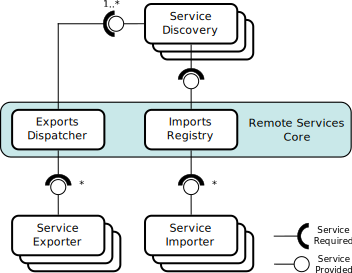
\includegraphics{../imgs/rs_arch}
\end{frame}

\begin{frame}{Remote Services Services}
\begin{exampleblock}{Note}
All services names are declared in \texttt{pelix.remote}
\end{exampleblock}

\begin{block}{Core Services}
\begin{small}
\begin{tabular}{rp{.55\textwidth}}
\texttt{\scriptsize SERVICE\_DISPATCHER} & Read-only access to the list of export endpoints \\
\texttt{\scriptsize SERVICE\_DISPATCHER\_SERVLET} & Utility methods for HTTP-based discovery \\
\texttt{\scriptsize SERVICE\_REGISTRY} & Write-only access to the list of import endpoints \\
\end{tabular}
\end{small}
\end{block}

\begin{block}{Import/Export Services}
\begin{small}
\begin{tabular}{rp{.45\textwidth}}
\texttt{\scriptsize SERVICE\_EXPORT\_PROVIDER} & Notified by the dispatcher to create export endpoints \\
\texttt{\scriptsize SERVICE\_EXPORT\_ENDPOINT\_LISTENER} & Notified of new export endpoints \\
\texttt{\scriptsize SERVICE\_IMPORT\_ENDPOINT\_LISTENER} & Notified of new import endpoints \\
\end{tabular}
\end{small}
\end{block}
\end{frame}

\begin{frame}{Endpoint creation sequence}
\begin{small}
\begin{block}{Service export/import}
The \texttt{Dispatcher} is notified of a service to be exported (after its registration or update), notifies the exporters and notifies the discovery services about the created endpoints.
\end{block}
\end{small}

\vspace{2ex}

\centering
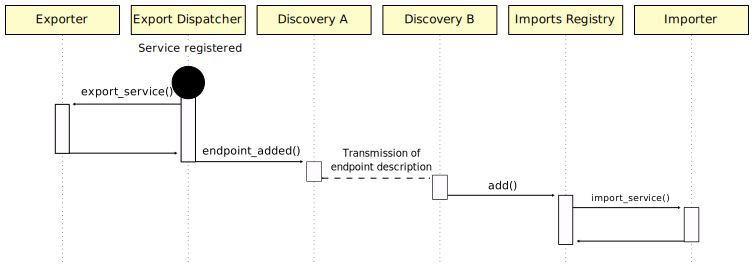
\includegraphics[width=\textwidth]{../imgs/rs_sequence}
\end{frame}
